\documentclass[10pt]{article}

%\usepackage[latin1]{inputenc}
%\usepackage[english]{babel}
\usepackage{graphicx}
\usepackage{color}
\usepackage{amsmath}
\usepackage{amssymb}
\usepackage{hyperref}
\usepackage{pbox}

\setlength{\parindent}{0cm}

\oddsidemargin -0in%5mm
\evensidemargin -0in%5mm
\topmargin -0.7in%-0.8in%-10mm
%\textheight 9.5in%9.5in%230mm
\textheight 9.2in
\textwidth 6.4in%150mm

%\pagestyle{empty} 

\begin{document}

%\hyphenpenalty=10000
%\sloppy

\hyphenation{}


\newcommand{\lkon}{\begin{color}{blue}}
\newcommand{\lkoff}{\end{color}}

\newcommand{\spc}{\vspace*{0.5cm}}
\newcommand{\spcp}{\vspace*{0.2cm}}

\newcommand{\tsize}{\large}

\newcommand{\ug}{$^*$}
\newcommand{\ugshift}{\hspace*{-0.835cm}}
\newcommand{\gr}{$^\dagger$}
\newcommand{\grshift}{\hspace*{-0.835cm}}

\vspace*{-0.3in}
\makebox[1.072\linewidth][c]
{
%\begin{figure}
  %\vspace{-0.3in}
%\hspace{-1cm}
%\begin{minipage}{0.3\columnwidth}
%\flushleft
%\includegraphics[height=0.8in,trim = 7.295cm 3.53cm 1.24cm 1.18cm, clip]%0.9in]
%{CSUF_logo}
%\end{minipage}
%\hfill
\begin{minipage}{0.5\columnwidth}
  %\flushright {\LARGE Alain Plattner}\\
  \centering {\LARGE Alain Plattner}\\
  \lkon\url{amplattner@ua.edu}\lkoff\\
  \lkon\url{http://alainplattner.net}\lkoff\\
\end{minipage}
%\hfill
%\hspace*{1cm}
%\begin{minipage}{0.3\columnwidth}
%  \flushright
%  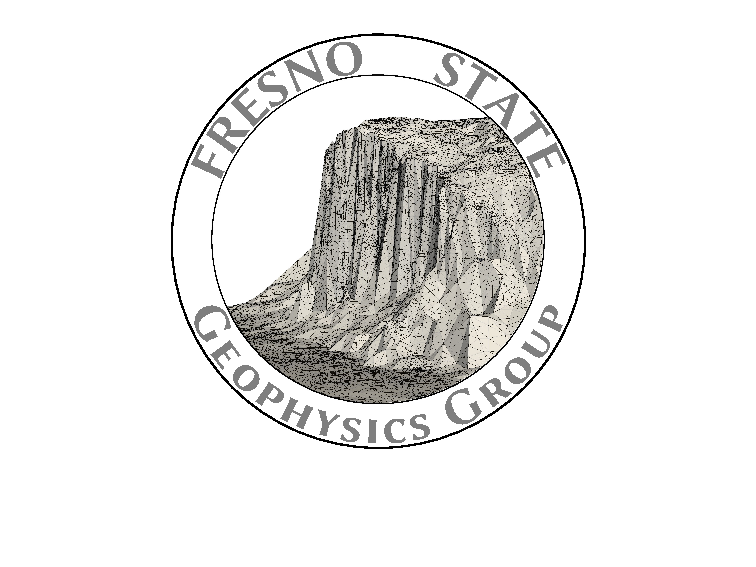
\includegraphics[height=0.8in,trim = 2.85cm 2cm 2.85cm 0.5cm,clip]{FSGG_logo}
%\end{minipage}
%\end{figure}
}



\vspace*{1cm}
\textbf{\tsize CV date:} {\tsize \today}

\spcp
For the most recent version of my \href{http://alainplattner.net/downloads/Plattner_CV.pdf}{CV} click \href{http://alainplattner.net/downloads/Plattner_CV.pdf}{\lkon\underline{here}\lkoff}

\spc
\textbf{\tsize Expertise:}

\spcp
Planetary crustal magnetic fields. Regional
  inversion of satellite magnetic data. Regional spherical-harmonic spectral
  analysis.  Electrical resistivity tomography. Near-surface geophysics.  

\spc
\textbf{\tsize Address:}

\spcp
Department of Geological Sciences\\
University of Alabama\\
Box 870338\\
Tuscaloosa, AL 35487, USA

%% \spcp
%% Department of Earth and Environmental Sciences\\
%% California State University, Fresno\\
%% 2576 E. San Ramon Ave., Mail Stop ST-24\\
%% Fresno, CA 93740


\spc
\textbf{\tsize Positions:}

\spcp
2018--present:
Assistant Professor at the Department of Geological Sciences, \\University of Alabama, Tuscaloosa AL, USA

\spcp
2014--2018:
Assistant Professor at the Department of Earth and Environmental Sciences, \\California State University Fresno, Fresno CA, USA

\spcp
2011--2014:
Postdoctoral Researcher at the Department of Geosciences, \\Princeton University, Princeton NJ, USA
%Research topic: Development of vectorial Slepian functions and their application to the estimation of crustal magnetization from satellite data.


\spc
\textbf{\tsize Degrees:}

\spcp
\par{2011:} PhD (Dr. Sc. ETH Zurich) in Geophysics at the Institute of Geophysics,
ETH Zurich, Switzerland.
Thesis title: \emph{ Adaptive wavelet methods for geoelectric modelling and inversion}.
Adviser: Prof. Hansruedi Maurer.
doi: 10.3929/ethz-a-006481159

\spcp
\par{2006:} Master of Science in Mathematics at the Institute of Mathematics,
 University of Basel, Switzerland.
 Majors: Algebraic geometry, numerical mathematics

 \spcp
\par{ 2004:} Bachelor of Science in Mathematics at the Institute of Mathematics, 
University of Basel, Switzerland.


\spc
\textbf{Honors and Awards:}

\spcp
NASA Planetary Science Early Career Award (ECA2019, received in April 2020)


\spc
\textbf{\tsize Publications:}

\spcp
\ug: Undergraduate student first author\\
\gr: Graduate student first author

\spcp
\emph{Research articles/book chapters:}


\spcp
%\hspace{-0.33cm}\gr \,
\grshift\gr[12] M.~Pacheco, \textbf{A.~Plattner}, G.~M.~Stock, D.~H.~Rood, C.~J.~Pluhar (2020), Surface exposure dating and geophysical investigation of the Royal Arches Meadow rock avalanche, Yosemite Valley, California, \emph{Front.~Earth~Sci}, 8:372, \href{https://pdfs.semanticscholar.org/5123/1ede4d8b8f76e2a2f2d2603595d307d09233.pdf}{doi: 10.3389/feart.2020.00372}


\spcp
\hspace{-0.675cm}[11] \textbf{A.~Plattner} (2020), GPRPy: Open-source ground penetrating radar processing and visualization \\software, \emph{The Leading Edge}, 39(5):298--368, \href{https://library.seg.org/doi/abs/10.1190/tle39050332.1}{doi: 10.1190/tle39050332.1}

\clearpage

\spcp
\ugshift\ug[10] A.~R.~Robbins, \textbf{A.~Plattner} (2018),
Offset-electrode profile acquisition strategy for
electrical resistivity tomography,
\emph{J.~Appl.~Geoph.}, 151:66--72, \href{https://www.sciencedirect.com/science/article/pii/S0926985117308376?via%3Dihub}{doi:~10.1016/j.jappgeo.2018.01.027} 


\spcp
\hspace{-0.5cm}[9] \textbf{A.~Plattner}, F.~J.~Simons (2017),
Internal and external potential field estimation
from regional gradient data at varying satellite altitude,
\emph{Geophys.~J.~Int.}, 211(1):207--238, \href{https://academic.oup.com/gji/article-lookup/doi/10.1093/gji/ggx244}{doi:~10.1093/gji/ggx244} 

\spcp
\hspace{-0.5cm}[8] \textbf{A.~Plattner}, F.~J.~Simons (2015),
High-resolution local magnetic field models for the
Martian South Pole
from Mars Global Surveyor data,
\emph{J.~Geophys.~Res.}, 120:1543--1566,
\href{http://onlinelibrary.wiley.com/doi/10.1002/2015JE004869/abstract}{doi: 10.1002/2015JE004869}

\spcp
\hspace{-0.5cm}[7] C.~Harig, K.~W.~Lewis, \textbf{A.~Plattner}, and F.~J.~Simons (2015),
A suite of software analyzes data on the sphere,
\emph{Eos Trans.~AGU}, 96(6):18--22,
\href{https://eos.org/project-updates/a-suite-of-software-analyzes-data-on-the-sphere-2}{doi: 10.1029/2015EO025851}

\spcp
\hspace{-0.5cm}[6] \textbf{A.~Plattner} and F.~J.~Simons (2015),
Potential field estimation using scalar and vector Slepian functions at satellite altitude,
\emph{Handbook of Geomathematics, 2nd edition},
\href{https://link.springer.com/referenceworkentry/10.1007\%2F978-3-642-27793-1_64-2}{doi: 10.1007/978-3-642-27793-1\_64-2}

\spcp
\hspace{-0.5cm}[5] F.~J.~Simons and \textbf{A.~Plattner} (2015),
Scalar and vector Slepian functions, spherical signal estimation and spectral analysis,
\emph{Handbook of Geomathematics, 2nd edition},
\href{https://link.springer.com/referenceworkentry/10.1007\%2F978-3-642-27793-1_30-2}{doi: 10.1007/978-3-642-27793-1\_30-2}

\spcp
\hspace{-0.5cm}[4] \textbf{A.~Plattner} and F.~J.~Simons (2014),
Spatiospectral concentration of vector fields on a sphere,
\emph{Appl.~Comput.~Harmon.~Anal.}, 36(1):1--22, 
\href{http://www.sciencedirect.com/science/article/pii/S106352031300002X?via\%3Dihub}{doi: 10.1016/j.acha.2012.12.001}

\spcp
\hspace{-0.5cm}[3] \textbf{A.~Plattner} and F.~J.~Simons (2013), 
A spatiospectral localization approach for analyzing and repres enting vector-valued functions on spherical surfaces,
\emph{Proc. SPIE} 8858, Wavelets and Sparsity XV, 88580N,
\href{http://proceedings.spiedigitallibrary.org/proceeding.aspx?articleid=1745029}{doi: 10.1117/12.2024703}

\spcp
\hspace{-0.5cm}[2] \textbf{A.~Plattner}, H.~R.~Maurer, J.~Vorloeper and M.~Blome (2012),
3-D electrical resistivity tomography using adaptive wavelet parameter grids,
\emph{Geophys.~J.~Int.}, 189(1):317--330,
\href{https://academic.oup.com/gji/article-lookup/doi/10.1111/j.1365-246X.2012.05374.x}{doi: 10.1111/j.1365-246X.2012.05374.x}

\spcp
\hspace{-0.5cm}[1] \textbf{A.~Plattner}, H.~R.~Maurer, J.~Vorloeper and W.~Dahmen (2010),
Three-dimensional geoelectric modelling with optimal work/accuracy rate 
using an adaptive wavelet algorithm,
\emph{Geophys.~J.~Int.}, 182(2):741--752,
\href{https://academic.oup.com/gji/article-lookup/doi/10.1111/j.1365-246X.2010.04677.x}{doi: 10.1111/j.1365-246X.2010.04677.x}

\spc
\emph{Extended abstracts:}

\spcp
\hspace{-0.67cm}\gr[8] A.~C.~Mills, \textbf{A.~Plattner} (2020), Regional Power Spectral
Estimation with Application to Galileo Data of Ganymede, \emph{51th
  Lunar and Planetary Science Conference 2019},
\href{https://www.hou.usra.edu/meetings/lpsc2020/pdf/2264.pdf}{Abstract
  2264}


\spcp
\hspace{-0.5cm}[7] \textbf{A.~Plattner}, C.~L.~Johnson (2019), Large-Scale Non-Axisymmetric Internal Structure of Mercury's Magnetic Field,
\emph{50th Lunar and Planetary Science Conference 2019},
\href{https://www.hou.usra.edu/meetings/lpsc2019/pdf/1645.pdf}{Abstract 1645}


\spcp
\hspace{-0.5cm}[6] \textbf{A.~Plattner}, C.~L.~Johnson (2018),
Regional Modeling and Power Spectra of Mercury's Crustal Magnetic Field,
\emph{Mercury 2018},
\href{https://www.hou.usra.edu/meetings/mercury2018/pdf/6023.pdf}{Abstract 6023}

\spcp
\hspace{-0.5cm}[5] C.~L.~Johnson,
\textbf{A.~M.~Plattner}. R.~J.~Phillips, L.~C.~Philpott, M.~Kinczyk,
L.~Prockter (2018), The Distribution and Origin of Mercury's Lithospheric Magnetization, \emph{Mercury 2018},
\href{https://www.hou.usra.edu/meetings/mercury2018/pdf/6052.pdf}{Abstract
  6052}

\spcp
\hspace{-0.5cm}[4] \textbf{A.~Plattner}, G.~J.~Golabek, F.~J.~Simons (2017),
A spectral view of the Terra Sirenum / Cimmeria crustal magnetic
field,
\emph{48th Lunar and Planetary Science Conference 2017},
\href{http://www.lpi.usra.edu/meetings/lpsc2017/pdf/1627.pdf}{Abstract 1627}

\spcp
\hspace{-0.67cm}\ug[3] A.~R.~Robbins and \textbf{A.~Plattner}
(2017),
2.75-D ERT: Zigzag electrode acquisition strategy to improve 2-D
Profiles,
\emph{Symposium on the Application of Geophysics to Engineering and
  Environmental Problems 2017}, 183--187,
\href{http://library.seg.org/doi/pdf/10.4133/SAGEEP.30-007}{doi: 10.4133/SAGEEP.30-007}

\spcp
\hspace{-0.5cm}[2] \textbf{A.~Plattner} and F.~J. Simons (2015),
Mars' heterogeneous South Polar magnetic field revealed using altitude vector Slepian functions,
\emph{46th Lunar and Planetary Science Conference 2015},
\href{http://www.hou.usra.edu/meetings/lpsc2015/pdf/1794.pdf}{Abstract 1794}

\spcp
\hspace{-0.5cm}[1] \textbf{A.~Plattner}, F.~J.~Simons, L.~Wei (2012),
Analysis of real vector fields on the sphere using Slepian functions,
\emph{IEEE Statistical Signal Processing Workshop (SSP)},
\href{http://ieeexplore.ieee.org/stamp/stamp.jsp?tp=&arnumber=6319659}{Abstract}

%\spc
\clearpage
\emph{Non peer-reviewed publications:}

\spcp
\hspace{-0.5cm}[1] \textbf{A.~Plattner}, M.~Pacheco, (2019), A
community-developed free Ground Penetrating Radar software,
\emph{Near-Surface Views, Newsletter of the Near-Surface Geophysics
  Technical Section of The Society of Exploration Geophysicists},
\href{https://seg.org/Portals/0/SEG/News%20and%20Resources/Near%20Surface/Near%20Surface%20Newsletter/2011-present/2019_Q1.pdf}{Q1
  2019 Newsletter}



\spc
\textbf{\tsize Talks:}

\spcp
\ug: Undergraduate student first author\\
\gr: Graduate student first author

\spcp
\emph{Invited/solicited conference talks:} 

\spcp 
\hspace{-0.4cm} \ug \hspace{-0.03cm} 2.75-D ERT: Zigzag electrode acquisition strategy
to improve 2-D profiles,
A.~R.~Robbins, A.~Plattner,
\emph{23rd European Meeting of Environmental and Engineering Geophysics}, Malmo, Sweden, Sep 2017 (best of SAGEEP)

\spcp
High-resolution crustal magnetic field model of the Martian South Pole using altitude vector\\ Slepian functions,
A.~Plattner, F.~J.~Simons,
\emph{Joint Mathematics Meeting}, San Antonio, TX, Jan 2015 (invited)

\spcp
Planetary potential-field inversion from vectorial data: Using Slepian functions for varying satellite altitude,
A.~Plattner, F.~J.~Simons,
\emph{Joint Mathematics Meeting}, Baltimore, MD, Jan 2014 (invited)

\spcp
Regional crustal field modeling from regional satellite data with varying altitude using dedicated vector Slepian functions,
A.~Plattner, F.~J.~Simons,
\emph{AGU Fall Meeting}, San Francisco, CA, Dec 2013 (invited)

\spcp
Signal and Spectral Estimation on a Sphere,
F.~J.~Simons, A.~Plattner,
\emph{AMMCS 2013}, Waterloo, ON, Canada, August 2013 (invited speaker: F.J.~Simons)

\spcp
Vectorial Slepian functions and the estimation of the crustal magnetic field,
A.~Plattner, F.~J.~Simons,
\emph{EGU General Assembly}, Vienna, Austria, April 2013 (solicited)

\spc
\emph{Regular conference talks:}

\spcp
Non-axisymmetric structure in Mercury's core field, A.~Plattner, C.~L.~Johnson,\emph{Mercury Exploration Assessment Group meeting 2021 (MExAG21)}, online, Feb 2021 

\spcp
\hspace{-0.4cm} \gr \hspace{-0.03cm} Three-dimensional Geophysical Imaging of the Royal Arches Meadow Rock Avalanche in Yosemite Valley, California, M.~Pacheco, A.~Plattner, G.~Stock, C.~Pluhar, \emph{AGU Fall Meeting}, San Francisco, CA, Dec 2019

\spcp
Mercury's Large-Scale Non-Axisymmetric Internal Field from MESSENGER Data, A.~Plattner, C.~L.~Johnson, \emph{AGU Fall Meeting}, San Francisco, CA, Dec 2019

\spcp
Large-Scale Non-Axisymmetric Internal Structure or Mercury's Magnetic Field,
A.~Plattner, C.~L.~Johnson, \emph{50th Lunar and Planetary Science Conference},
The Woodlands, TX, March 2019

\spcp
A spectral view of the Terra Sirenum / Cimmeria crustal magnetic field, A.~Plattner, F.J.~Simons, G.~Golabek, \emph{48th Lunar and Planetary Science Conference}, The Woodlands, TX, March 2017

\spcp 
\hspace{-0.4cm} \ug \hspace{-0.03cm}  2.75-D ERT: Zigzag electrode acquisition strategy
to improve 2-D profiles,
A.~R.~Robbins, A.~Plattner,
\emph{SAGEEP}, Denver, CO, Mar 2017

\spcp
The Crustal Magnetic Field of Terra Sirenum and Cimmeria, Mars. A Spectral Perspective,
A.~Plattner, F.~J.~Simons, G.~Golabek, 
\emph{AGU Fall Meeting}, San Francisco, CA, Dec 2016

\spcp
Teaching Near-Surface Geophysics within the Matlab/Octave Community,
A.~Plattner, 
\emph{AGU Fall Meeting}, San Francisco, CA, Dec 2016

\spcp
Localized Bandlimited Inversion of Planetary Magnetic-Field Data,
A.~Plattner, F.~J.~Simons,
\emph{SIAM Conference on Mathematical and Computational Issues in the Geosciences},
Stanford University, Stanford, CA, Jul 2015

\spcp
Source field estimation from satellite data using vectorial spatiospectrally 
concentrated functions,
A.~Plattner, F.~J.~Simons,
\emph{Geomathematics 2013}, Sankt Martin, Germany, April 2013

\clearpage
\spcp
Vector-valued crustal magnetic field estimation using vector Slepian functions,
A.~Plattner, F.~J.~Simons,
\emph{AGU Fall Meeting}, San Francisco, CA, Dec 2012

\spcp
Geophysical survey of the Peristeries plateau in Polis Chrysochous, Cyprus,
A.~Plattner, F.~J.~Simons, J.~S.~Smith, A.~C.~Maloof, J.~Husson,
\emph{American Schools of Oriental Research Annual Meeting}, Chicago, IL, Nov 2012

\spcp
Adaptive wavelet parameterization for 3d electrical resistivity tomography,
A.~Plattner, H.~R.~Maurer, 
\emph{AGU Fall Meeting}, San Francisco, CA, Dec 2011

\spcp
Adaptive wavelet modeling of geophysical data,
A.~Plattner, H.~R.~Maurer, J.~Vorloeper and W.~Dahmen, 
\emph{AGU Fall Meeting}, San Francisco, CA, Dec 2009


\spc
\emph{Webinar talks:}

\spcp
Examples using Matlab / Octave for Experimental Design and Data Processing in a Near-surface Applied Geophysics Class, 
\emph{Developing Computational Skills in the Sciences with Matlab}, April 2017\\
\url{http://serc.carleton.edu/details/files/115169.html}

\spc
\emph{Seminar talks:}\\
\emph{University of South Florida, School of Geosciences, Feb 2020}\\
\emph{University of Mississippi, Department of Geology and Geological Engineering, Oct 2019}\\
\emph{University of Alabama, Department of Physics and Astronomy, Sep 2019}\\
\emph{University of Cape Town (South Africa), Department of Geology, Sep 2018}\\
\emph{NASA Goddard Space Flight Center (USA), July 2018}\\
\emph{University of Siegen (Germany), Department of Mathematics, May 2018}\\
\emph{University of Alabama, Department of Geological Sciences, Feb 2018}\\
\emph{University of the Witwatersrand (South Africa), School of Geosciences}, July 2016\\
\emph{University of British Columbia (CA), Dept.~of Earth, Ocean and Atmospheric Sci.}, Feb 2016\\
\emph{UC Santa Cruz (USA), Earth and Planetary Sciences Department}, Oct 2014\\
\emph{Princeton University (USA), Department of Geosciences}, Sept  2011, Apr 2014\\
\emph{CSU Fresno (USA), Department of Earth and Environmental Science}, Feb 2014\\
\emph{Princeton University (USA), Program in Appl.~and Comp.~Mathematics}, Nov 2013\\
\emph{Rutgers (USA), Department of Earth and Environmental Sciences}, Feb 2012\\
\emph{Cornell University (USA), Department of Earth and Atmospheric Sciences}, Feb 2012\\
\emph{Universite de Lausanne (Switzerland), Institute de Geophysique}, Nov 2009, Jan 2012\\
\emph{ETH Zurich (Switzerland), Seminar for Applied Mathematics}, Dec 2010\\
\emph{ETH Zurich (Switzerland), Department of Earth Sciences}, Oct 2009

%\clearpage
\spc
\textbf{\tsize Posters:}

\spcp
\ug: Undergraduate student first author\\
\gr: Graduate student first author

\spcp
\emph{Invited conference posters:}

\spcp
Ground Penetrating Radar Data Processing and Visualization using
GPRPy,
A.~Plattner,
\emph{AGU Fall Meeting}, Washington DC, Dec 2018 


\spcp
\emph{Regular conference posters:}

\spcp
Local power spectrum from local data,
A.~Plattner, C.~L.~Johnson,
\emph{AGU Fall Meeting}, San Francisco CA / online, Dec 2020

\spcp
\hspace*{-0.4cm} \gr \, Geophysical Investigation of the Royal Arches Meadow Rock
Avalanche in Yosemite Valley - CA,
M.~Pacheco, A. Plattner,
\emph{GSA Cordilleran Meeting}, Portland OR, May 2019

\clearpage

\spcp
Mercury's Core Field: Beyond the Offset Axial Dipole,
A.~Plattner, C.~L.~Johnson, 
\emph{AGU Fall Meeting}, Washington DC, Dec 2018 

\spcp
\hspace*{-0.45cm} \gr \hspace*{-0.05cm} Near Surface Geophysical Imaging of the Internal
Structure of El Capitan Meadow Rock Avalanche in Yosemite National
Park, California,
C.~Liu, A.~Plattner, G.~Stock,
\emph{AGU Fall Meeting}, Washington DC, Dec 2018


\spcp
Mercury's Crustal Magnetic Field from MESSENGER Data,
 A.~Plattner, C.~L.~Johnson, 
\emph{AGU Fall Meeting}, New Orleans, LA, Dec 2017 

\spcp
\hspace{-0.42cm} $^*$ A glimpse in the third dimension for electrical
resistivity profiles,
A.~R.~Robbins, A.~Plattner,
\emph{AGU Fall Meeting}, New Orleans, LA, Dec 2017 

\spcp
\hspace{-0.38cm} $^*$ Electrical Resistivity and Ground Penetrating Radar 
Investigation of Presence and Extent of Hardpan Soil Layers,
 S.~J.~Thao, A.~Plattner,
\emph{AGU Fall Meeting}, San Francisco, CA, Dec 2015

\spcp
Localized crustal magnetic field inversion from inner- and outer-source altitude vector Slepian functions,
A.~Plattner,  F.~J.~Simons,
\emph{AGU Fall Meeting}, San Francisco, CA, Dec 2015

\spcp
Mars' Heterogeneous South Polar Magnetic Field Revealed using Altitude Vector Slepian Functions,
A.~Plattner,  F.~J.~Simons,
\emph{46th Lunar and Planetary Science Conference}, The Woodlands, TX, March 2015

\spcp
High-resolution Local Crustal Magnetic Field Modeling of the Martian South Pole,
A.~Plattner,  F.~J.~Simons,
\emph{AGU Fall Meeting}, San Francisco, CA, Dec 2014

\spcp
Altitude vector Slepian functions and satellite crustal magnetic field data,
A.~Plattner,  F.~J.~Simons,
\emph{3rd Swarm Science Meeting}, Copenhagen, Denmark, June 2014

\spcp
Local gravity field modeling from vectorial satellite data using Slepian functions,
A.~Plattner,  F.~J.~Simons,
\emph{AGU Fall Meeting}, San Francisco, CA, Dec 2013

\spcp
Analysis of real vector fields on the sphere using Slepian functions,
A.~Plattner, F.~J.~Simons, L.~Wei,
\emph{IEEE Statistical Signal Processing Workshop}, Ann Arbor, MI, Aug 2012

\spcp
Lithospheric magnetic field reconstruction using vector Slepian functions,
A.~Plattner, F.~J.~Simons,
\emph{Symposium on Study of the Earth's Deep Interior}, Leeds, United Kingdom, July 2012

\spcp
Spatiospectral concentration of vector fields on a sphere,
A.~Plattner, F.~J.~Simons,
\emph{Challenges in Geometry, Analysis, and Computation: High-Dimensional Synthesis}, 
New Haven, CT, June 2012

\spcp
Vector spherical Slepian functions -- spatiospectral concentration of vector fields on the sphere,
A.~Plattner, F.~J.~Simons, L.~Wei,
\emph{AGU Fall Meeting}, San Francisco, CA, Dec 2011


\spc
\textbf{\tsize Teaching:}

\spcp
\textbf{2021}

``The Dynamic Earth'', Department of Geological Sciences, University of Alabama

\spcp
\textbf{2020, 2019}

``Introduction Geophysics'', Department of Geological Sciences,
University of Alabama

``Hazardous Earth'', Department of Geological Sciences, University of Alabama

``The Dynamic Earth'', Department of Geological Sciences, University of Alabama

\spcp
\textbf{2018}

``Hazardous Earth'', Department of Geological Sciences, University of Alabama

\spcp
\textbf{2017}

``Applied Geophysics'', Department of Earth and Environmental Science, CSU Fresno.

``Natural Disasters and Earth Resources'', Department of Earth and Environmental Science, CSU Fresno.

\clearpage
\spcp
\textbf{2016}

``Geoscientific Computing'', Department of Earth and Environmental Science, CSU Fresno.

``Natural Disasters and Earth Resources'', Department of Earth and Environmental Science, CSU Fresno.

\spcp
\textbf{2015}

``Near-surface geophysics'', Department of Earth and Environmental Science, CSU Fresno.

``Natural Disasters and Earth Resources'', Department of Earth and Environmental Science, CSU Fresno.

\spcp
\textbf{2014}

``Geophysics Seminar'', Department of Earth and Environmental Science, CSU Fresno.

``Environmental Earth and Life Science'', Department of Earth and Environmental Science, CSU Fresno.

\spcp
\textbf{2011--2013}

Instructor for Earth's environments and ancient civilizations'', Department of Geosciences,\\ Princeton University.

\spcp
\textbf{2006--2011}

Teaching assistant for Numerical modeling in applied geophysics'',  Institute of Geophysics, ETH Zurich.
     
Teaching assistant for field courses (electromagnetic prospecting),
Institute of Geophysics, ETH Zurich.

\spcp
\textbf{2004--2006}

Teaching assistant for ``Mathematics for natural scientists'', Institute of Mathematics, University of Basel.

\spcp
\textbf{2004}

Teaching assistant for ``Linear algebra'', Institute of Mathematics, University of Basel.

\spc
\textbf{\tsize Funding:}

\spcp
NASA Planetary Science Early Career Award [19-ECA19-0026], 2020--2023  

\spcp
NASA Discovery Data Analysis Program [80NSSC19K1426], 2019--2022

\spcp
  NSF Geoinformatics
  %\href{http://www.nsf.gov/awardsearch/showAward?\
  %  AWD_ID=1550732&HistoricalAwards=false}{\lkon[EAR-1550732]\lkoff},
  [EAR-1550732],
  2016--2020

 \spcp 
NASA Mars Data Analysis Program [NNX14AM29G], 2014--2017

\spcp
Swiss National Science Foundation Fellowship for Prospective Researchers
[PBEZP2-134427], 2011--2012

\spcp
Ulrich Schmucker Memorial Trust grant (2011)

\spc
\textbf{\tsize Advising:}

\spcp
PhD Students:\\
Ramon Richardson, expected 2024 (University of Alabama)

\spcp
Master's Students:\\
Michaela May, expected 2022 (University of Alabama)\\
Alyssa Mills, expected 2021 (University of Alabama)\\
Yagmur Yilmaz, expected 2021 (University of Alabama)\\
Marcus Pacheco, 2019 (California State University, Fresno)\\
Christine Liu, 2018 (California State University, Fresno)

\spcp
External PhD examiner:\\
Kathrin Seibert, 2018 (University of Siegen, Germany)\\
Timothy Wiese, 2012 (University of Adelaide, Australia)


\clearpage
\spc
\textbf{\tsize Service:}

\spcp
Editor for International Journal on Geomathematics (GEM), since 2019

\spcp Chaired NASA grant proposal review panel (2021)

\spcp NASA grant proposal review panelist on three panels (2020-2021)


\spcp
Principal organizer / chair of several AGU sessions (2016 -- 2019)

\spcp
Reviewed numerous papers for the following journals:\\
\emph{Earth-Sci.~Rev.},
\emph{Geophys.~J.~Int.},
\emph{Geophys.~Prospect.},
\emph{Geophysics},
\emph{IEEE T.~Signal Proces.},\\
\emph{Intern.~J.~Geomath.},
\emph{Int.~J.~Speleol.},
\emph{J.~Geodesy},
\emph{J.~Geophys.~Res.},
\emph{Mech.~Res.~Commun.},\\
\emph{Pure~Appl.~Geophys.},
\emph{J.~Appl.~Geophys.},
\emph{Icarus}

\spcp
Co-organized the minisymposium
``Forward and Inverse Problems in Geodesy, Geodynamics, and Geomagnetism''
at SIAM Conference on Mathematical and Computational Issues in the Geosciences, July 2015.

%\spcp
%Served on the College of Science and Mathematics curriculum committee at\\
%California State University, Fresno.

\spcp
Appeared on the radio show ``Science, a candle in the dark'' on KFCF´
\url{https://itunes.apple.com/us/podcast/science-candle-in-dark-podcast/id972796179}

\spcp
Presented at the local Caf\'e Scientifique
\url{https://valleycafesci.wordpress.com/}




%
%\cventry{Service:}
%{%Organizer of the brown-bag seminar of the Department of Geosciences, Princeton University.
%%
%Between Feb 2012 and June 2012 I organized the brown-bag seminar for the Department of Geosciences, Princeton University.
%}


\end{document}

